\section{Further numerical results}\label{further-sec}

By Theorem \ref{Zero}, one can verify the second hypothesis of Theorem \ref{ubc-0} when $X \geq \exp(C/t_0)$ for a large constant $C$.  If we ignore for sake of discussion the third hypothesis of Theorem \ref{ubc-0} (which turns out to be relatively easy to verify numerically in practice), this suggests that one can obtain a bound of the form $\Lambda \leq O(t_0)$ provided that one can verify the Riemann hypothesis up to a height $\exp(C/t_0)$.  In other words, if one has numerically verified the Riemann hypothesis up to a large height $T$, this should soon lead to a bound of the form $\Lambda \leq O \left( \frac{1}{\log T} \right )$.

Aside from improving the implied constant in this bound, it does not seem easy to improve this sort of implication without a major breakthrough on the Riemann hypothesis (such as a massive expansion of the known zero-free regions for the zeta function inside the critical strip).  We shall justify this claim heuristically as follows. Suppose that there was a counterexample to the Riemann hypothesis at a large height $T$, so that $H_0(2T + iy) = 0$ for some positive $y$, which for this discussion we will take to be comparable to $1$.  The Riemann von Mangoldt formula indicates that the number of zeroes of $H_0$ within a bounded distance of this zero should be comparable to $\log T$; the majority of these zeroes should obey the Riemann hypothesis and thus stay at roughly unit distance from our initial zero $2T+iy$.  Proposition \ref{dynam} then suggests that as time $t$ advances, this zero should move at speed comparable to $\log T$.  Thus one should not expect this zero to reach the real axis until a time comparable to $\frac{1}{\log T}$.  This heuristic analysis therefore indicates that it is unlikely that one can significantly improve the bound $\Lambda \leq O \left( \frac{1}{\log T} \right )$ without being able to exclude significant violations of the Riemann hypothesis at height $T$.

The table below collects some numerical results verifying the second two hypotheses of Theorem \ref{ubc-0} for larger values of $X$, and smaller values of $t_0,y_0$, than were considered in Section \ref{newup-sec}.  This leads to improvements to the bound $\Lambda \leq 0.22$ conditional on the assumption that the Riemann Hypothesis can be numerically verified beyond the height $T \approx 3.06 \times 10^{10}$ used in Section \ref{newup-sec}.  For instance, the final row of the table implies that one has the bound $\Lambda \leq 0.1$ assuming that the Riemann hypothesis is verified up to the height $T \approx 4.5 \times 10^{21}$.  Note that this is broadly consistent with the previous heuristic that the upper bound on $\Lambda$ is proportional to $\frac{1}{\log T}$.

\begin{table}[ht!]
  \begin{center}
    \caption{Conditional $\Lambda$ Results}
    \label{tab:table1}
    \begin{tabular}{l|r|r|r|c|r|c} % <-- Alignments: 1st column left, 2nd middle and 3rd right, with vertical lines in between
      $X$ & $t_{0}$ & $y_{0}$ & $\Lambda$ & $\textbf{Winding Number}$ & $N_{0}$ & $|f_t(x+iy)|$ lower bound\\
      \hline
      $2 \times 10^{12} + 129093$ & 0.198 & 0.15492 & 0.21 & 0 & 398942 & 0.0341\\
      $5 \times 10^{12} + 194858$ & 0.186 & 0.16733 & 0.20 & 0 & 630783 & 0.0376\\
      $2 \times 10^{13} + 131252$ & 0.180 & 0.14142 & 0.19 & 0 & 1261566 & 0.0349\\
      $6 \times 10^{13} + 123375$ & 0.168 & 0.15492 & 0.18 & 0 & 2185096 & 0.0377\\
      $3 \times 10^{14} + 188911$ & 0.161 & 0.13416 & 0.17 & 0 & 4886025 & 0.0369\\
      $2 \times 10^{15} + 122014$ & 0.153 & 0.11832 & 0.16 & 0 & 12615662 & 0.0532\\
      $7 \times 10^{15} + 68886$ & 0.139 & 0.14832 & 0.15 & 0 & 23601743 & 0.0350\\
      $6 \times 10^{16} + 156984$ & 0.132 & 0.12649 & 0.14 & 0 & 69098829 & 0.0307\\
      $6 \times 10^{17} + 88525$ & 0.122 & 0.12649 & 0.13 & 0 & 218509686 & 0.0347\\
      $9 \times 10^{18} + 35785$ & 0.113 & 0.11832 & 0.12 & 0 & 846284375 & 0.0318\\
      $2 \times 10^{20} + 66447$ & 0.102 & 0.12649 & 0.11 & 0 & 3989422804 & 0.0305\\
      $9 \times 10^{21} + 70686$ & 0.093 & 0.11832 & 0.1 & 0 & 26761861742 & 0.0321\\
    \end{tabular}
  \end{center}
\end{table}

The selection of parameters in this table proceeded as follows.  One first located parameters $t_0, y_0, N_0$ (with the quantity $\Lambda = t_0 + \frac{1}{2} y_0^2$ as small as possible) for which one could obtain a good lower bound for $f_{t_0}(x+iy_0)$ when $x=N_0$; we arbitrarily chose a target lower bound of $|f_{t_0}(x+iy_0)| \geq 0.03$ to provide an adequate safety margin.  From \eqref{ftxy} one had
\begin{equation}\label{ftxy-2}
 f_{t_0}(x+iy_0) = \sum_{n=1}^N \beta_n + O_{\leq}( |\gamma| |\sum_{n=1}^N \alpha_n| ) + O_{\leq}(\left( |\gamma| \sum_{n=1}^N n^{y_0} \frac{b_n^{t_0}}{n^\sigma} (n^{|\kappa|}-1) \right)
\end{equation}
where
$$ \beta_n \coloneqq \frac{b_n^{t_0}}{n^{\sigma+iT}}$$
and
$$ \alpha_n \coloneqq n^{y_0} \frac{b_n^{t_0}}{n^{\sigma+iT}}.$$
The final term on the right-hand side of \eqref{ftxy-2} can be estimated as in Section \ref{b-bound} and is negligible in practice.  To control the other two terms, we use the following lemma (which roughly speaking corresponds to a simplified version of the ``Euler 2 mollifier'' version of the ``Euler 5 mollifier'' analysis in Section \ref{b-bound}):

\begin{lemma}\label{trib2}  Let $\alpha_1,\dots,\alpha_N$ be complex numbers, and let $\beta_2$ be a number such that whenever $1 \leq n \leq N$ is even, $\beta_2 a_{n/2}$ lies on the line segment $\{ \theta \alpha_n: 0 \leq \theta \leq 1\}$ connecting 0 with $\alpha_n$.  Then we have the lower bound
$$ |1-\beta_2| \left|\sum_{n=1}^N \alpha_n\right| \geq 2 |\alpha_1| - (1-|\beta_2|) \sum_{n=1}^N |\alpha_n| - 2 |\beta_2| \sum_{N/2 < n \leq N} |\alpha_n|$$
and the upper bound
$$ |1-\beta_2| \left|\sum_{n=1}^N \alpha_n\right| \leq (1-|\beta_2|) \sum_{n=1}^N |\alpha_n| + 2 |\beta_2| \sum_{N/2 < n \leq N} |\alpha_n|.$$
\end{lemma}

\begin{proof} The quantity $|1-\beta_2| |\sum_{n=1}^N \alpha_n|$ can be written as
$$ \left|\sum_{n=1}^{2N} (1_{n \leq N} \alpha_n - 1_{2|n} \alpha_{n/2} \beta_2)\right|.$$
By the triangle inequality, this is bounded above by
$$ \sum_{n=1}^{2N} |1_{n \leq N} \alpha_n - 1_{2|n} \alpha_{n/2} \beta_2|$$
and below by
$$ 2 |\alpha_1| - \sum_{n=1}^{2N} |1_{n \leq N} \alpha_n - 1_{2|n} \alpha_{n/2} \beta_2|.$$
We have
$$ \sum_{n=1}^{2N} |1_{n \leq N} \alpha_n - 1_{2|n} \alpha_{n/2} \beta_2| = \sum_{n=1}^N |\alpha_n| - 1_{2|n} |\alpha_{n/2}| |\beta_2| + \sum_{n=N+1}^{2N} 1_{2|n} |\alpha_{n/2}| |\beta_2|$$
which we can rearrange as
$$ (1 - |\beta_2|) \sum_{n=1}^N |\alpha_n| + 2 |\beta_2| \sum_{N/2 < n \leq N} |\alpha_n|$$
and the claim follows.
\end{proof}

Using this lemma to lower bound $|\sum_{n=1}^N \beta_n|$ and upper bound $|\sum_{n=1}^N \alpha_n|$, and then using the triangle inequality, yields a lower bound on $|f_{t_0}(x+iy_0)|$ when $N=N_0$.  These quantities can be readily computed for many values of $t_0,y_0,N_0$, leading to an envelope for $\Lambda$ and $x \approx 4 \pi N_0^2$ that is depicted in Figure \ref{tradeoff}.

\begin{figure}[!ht]
  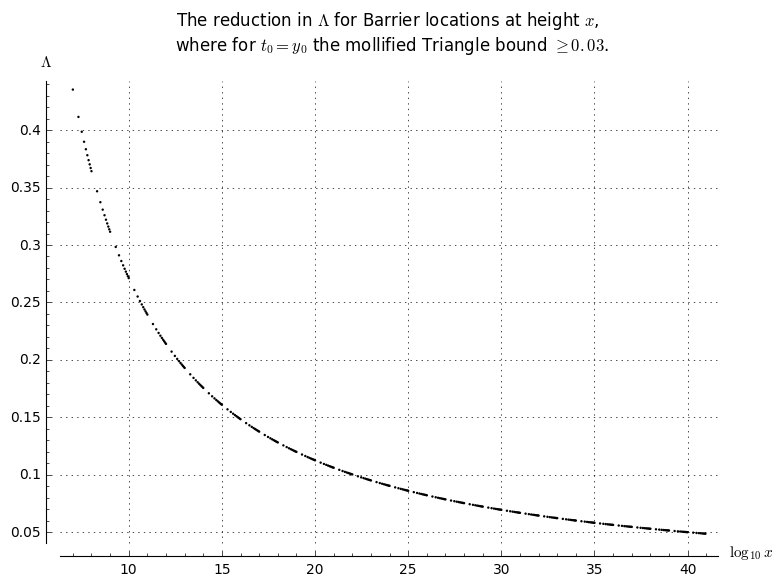
\includegraphics[width=1.0\linewidth]{tradeoff.png}
  \caption{The envelope of potential choices of $x, \Lambda$.  Note the approximate inverse relationship between $\Lambda$ and $\frac{1}{\log x}$.}
  \label{tradeoff}
\end{figure}

By working in intervals $N \in [N_-,N_+]$ for some finite number of intervals $[N_-,N_+]$ covering $[N_0,N_1]$ for some large $N_1$ as in Section \ref{b-bound}, and then using a crude triangle inequality bound for $N \geq N_1$ as in Section \ref{c-bound}, we thus (in view of the conservative safety margin in our lower bounds for $|f_{t_0}(x+iy_0)|$) expect to be able to verify the hypothesis in Theorem \ref{ubc-0}(iii) for any choice of parameters $t_0, y_0, N_0$ as above.  The main remaining difficulty is then to verify the barrier hypothesis (Theorem \ref{ubc-0}(ii)).  This is by far the most numerically intensive step, and we proceed as in Section \ref{barrier-sec}, after using the \emph{ad hoc} procedure in Section \ref{select} to select $X_0$.   The graphs in figure \ref{fig:meshbarrier} illustrate that for increasing $x$, the number of xy-rectangles to be evaluated within the barrier, as well as the number of mesh points required per rectangle (measured at $t=0$), increase exponentially. 

\begin{figure}[!ht]
  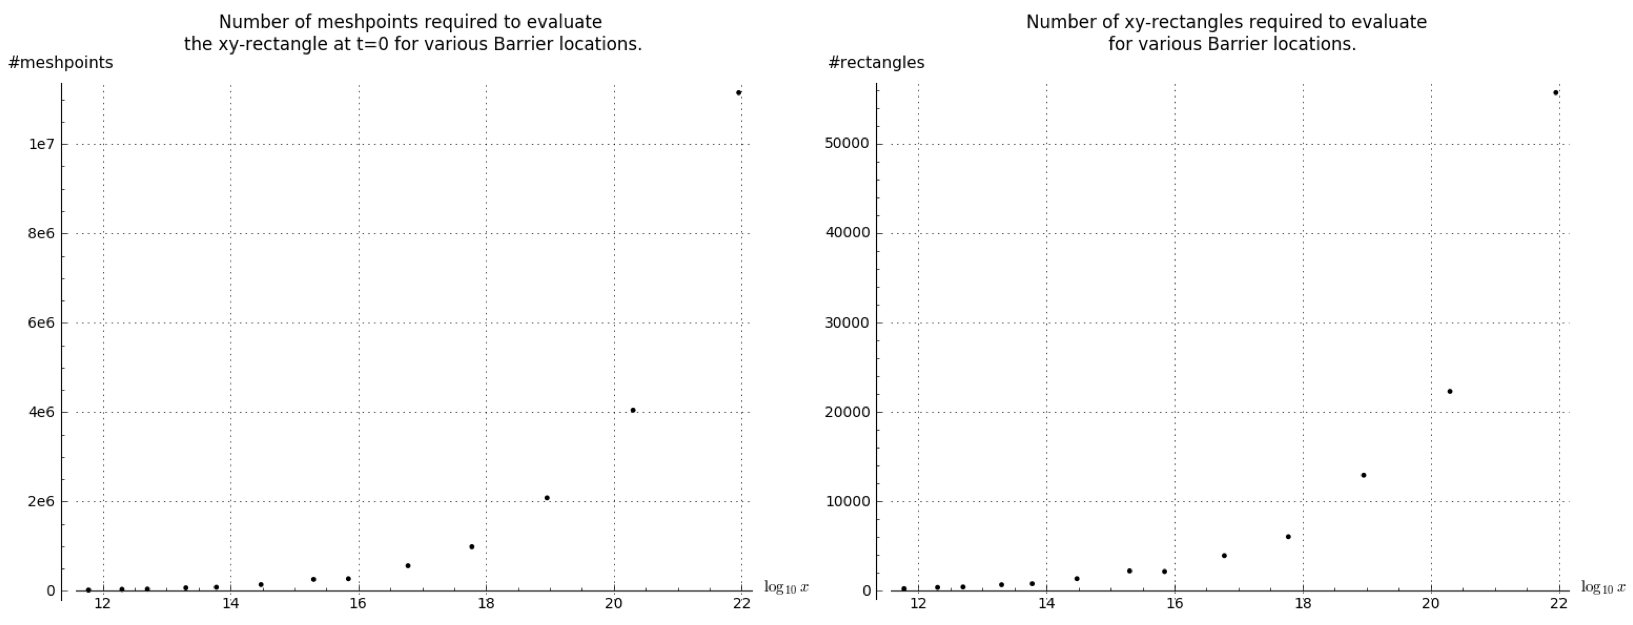
\includegraphics[width=1.0\linewidth]{mesh_rectangles_at_barrierlocs.png}
  \caption{The left graph shows how the number mesh points of the xy-rectangle at $t=0$ increases with $x$ for each barrier. The graph on the right does the same, but now for the total number of xy-rectangles that need to be evaluated per barrier. }
  \label{fig:meshbarrier}
\end{figure}

All barrier runs generated a winding number of zero for each rectangle and the scripts completed successfully without any errors. For all barrier locations, the computations of the mesh points where calculated at $20$ digits accuracy except for the highest two where $10$ digits where used (to be able to compute it within a reasonable time). Checks where made before each formal run to assure the target accuracy would be achieved. 

The computations for $X=2 \times 10^{20} + 66447$ and $X=9 \times 10^{21} + 70686$ in the above table were massive, and performed using a Boinc based grid computing setup, in which a few hundred volunteers participated. Their contributions can be tracked at {\tt anthgrid.com/dbnupperbound}.
